\newcommand{\mainfig}{
    \begin{figure}[ht!]
        \centering
        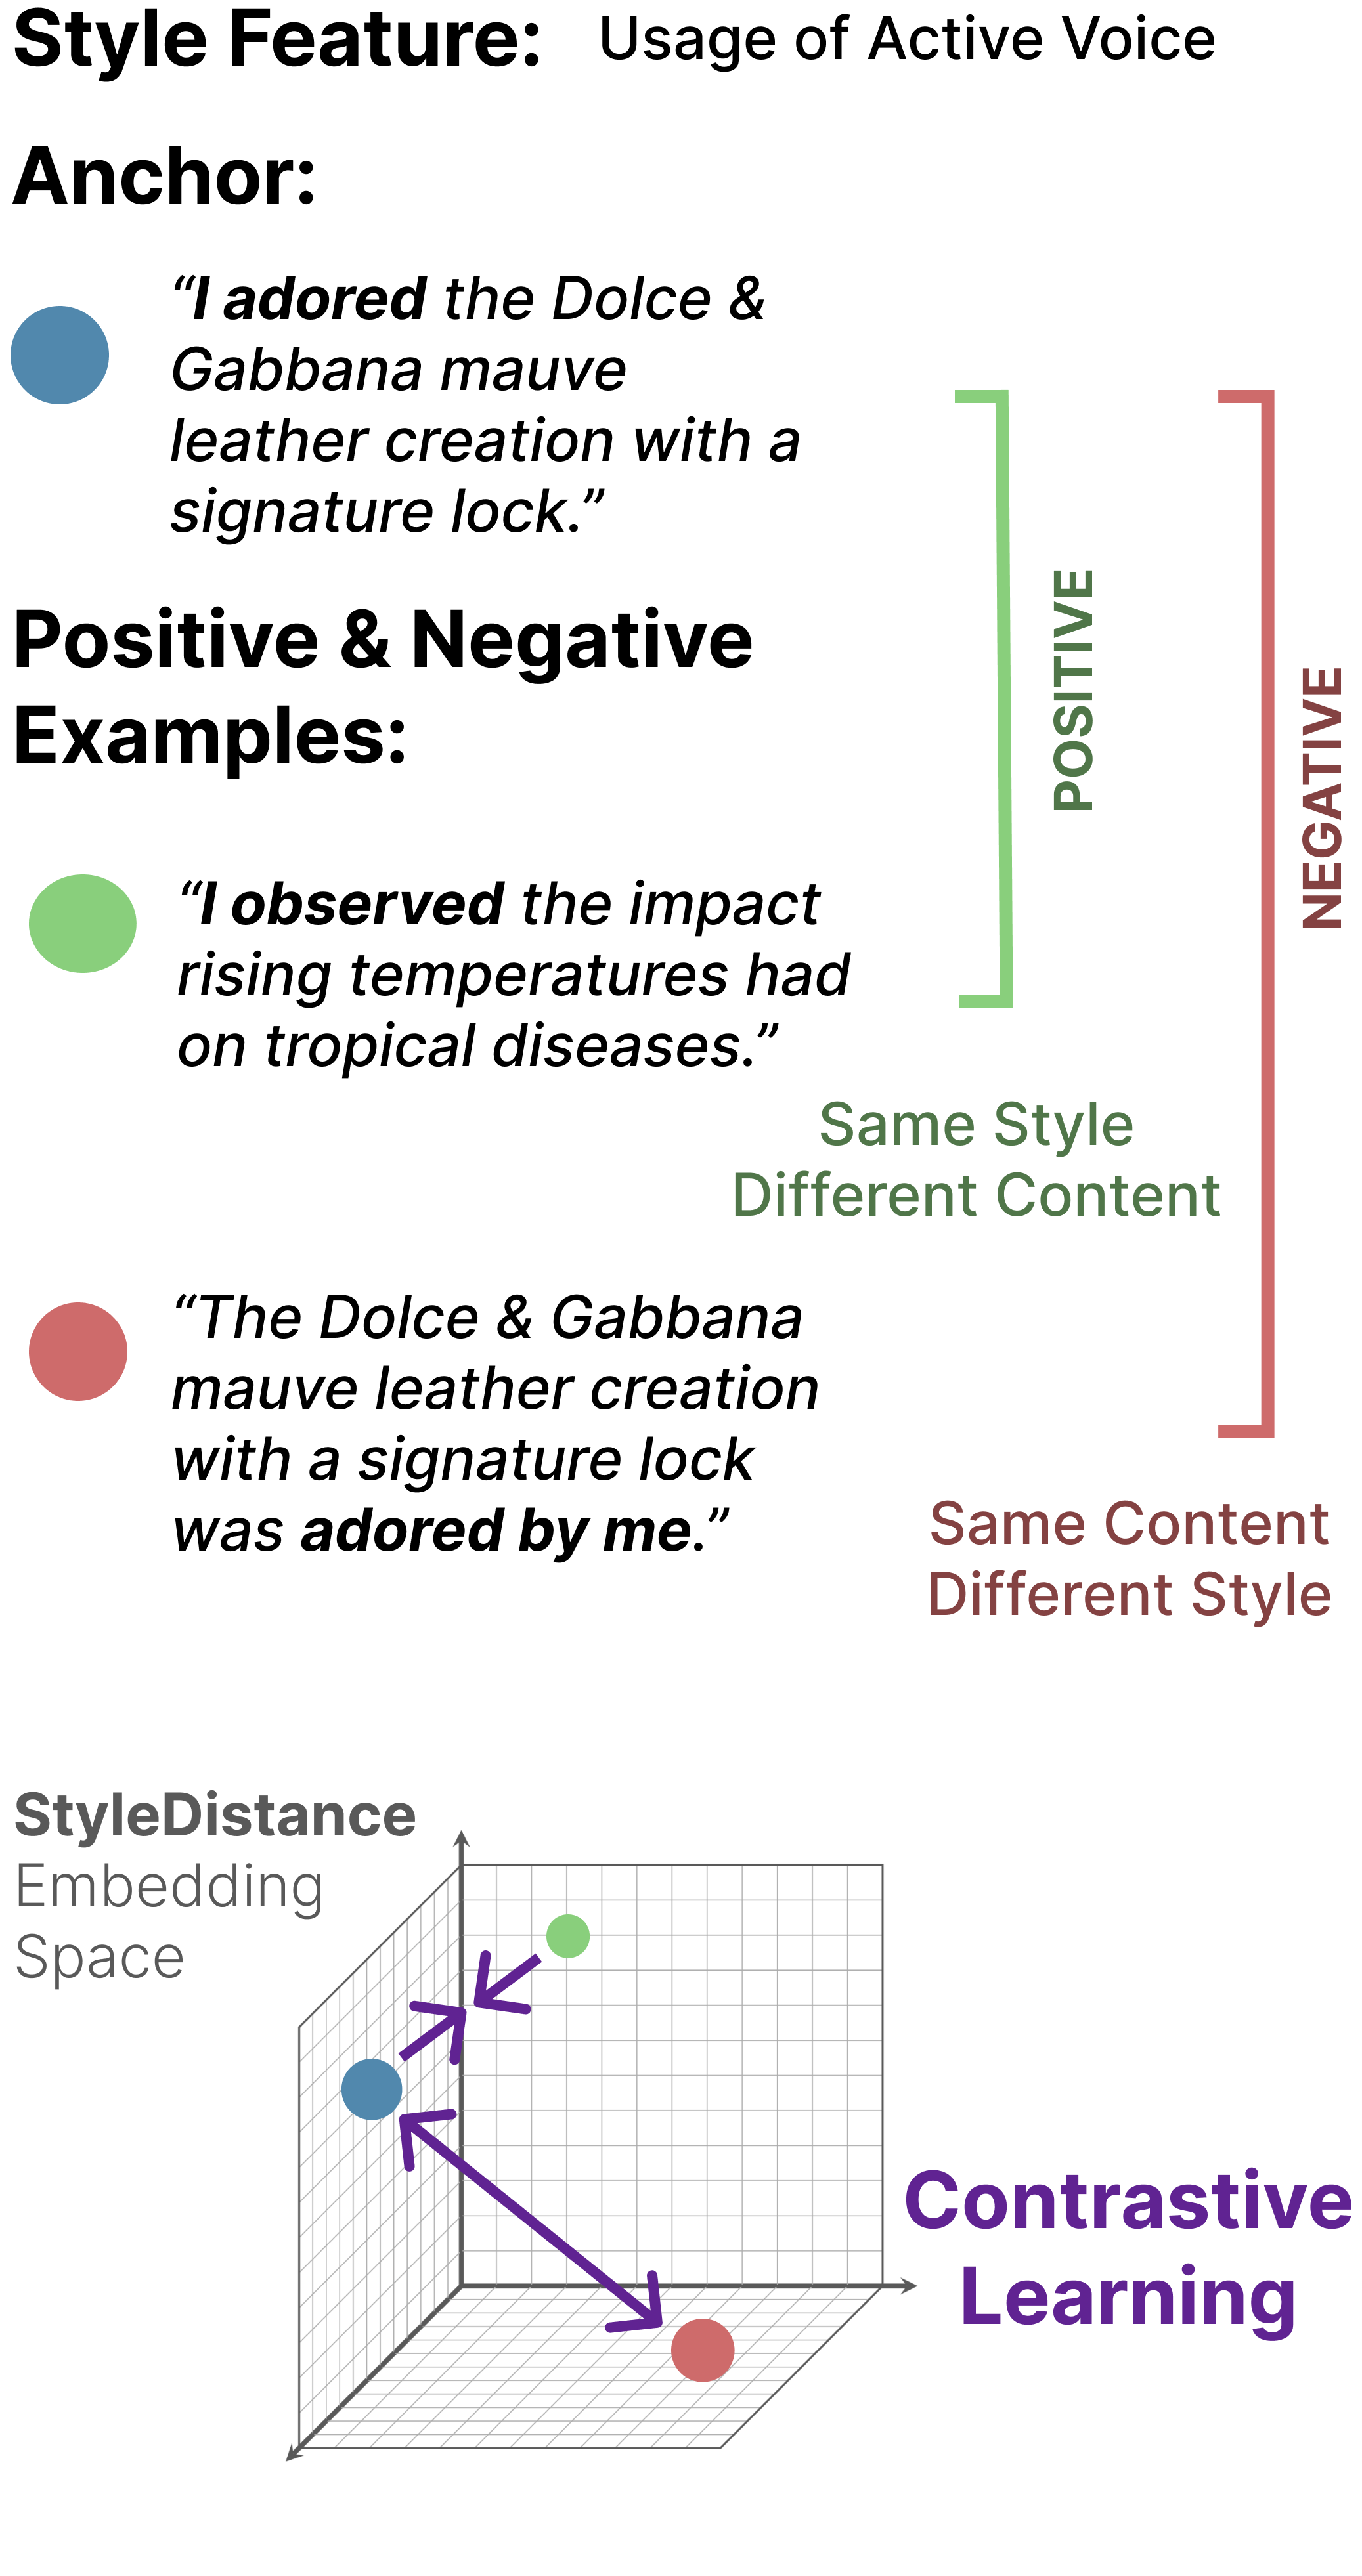
\includegraphics[width=185px]{resources/figures/StyleDistance.png}
        \caption{\textsc{StyleDistance} embeddings are trained using contrastive learning from synthetic parallel (positive and negative) examples %synthetically generated by a LLM that are positive and negative examples of usage of a style feature. The synthetic dataset % \textsc{StyleDistance} is trained on 
        % comprises of parallel examples for 
        representing 40  style features. The illustrated example is for the ``Usage of Active Voice'' feature.}
        \label{fig:main}
    \end{figure}
}

\newcommand{\mturkinterfacefig}{
    \begin{figure}[H]
        \centering
        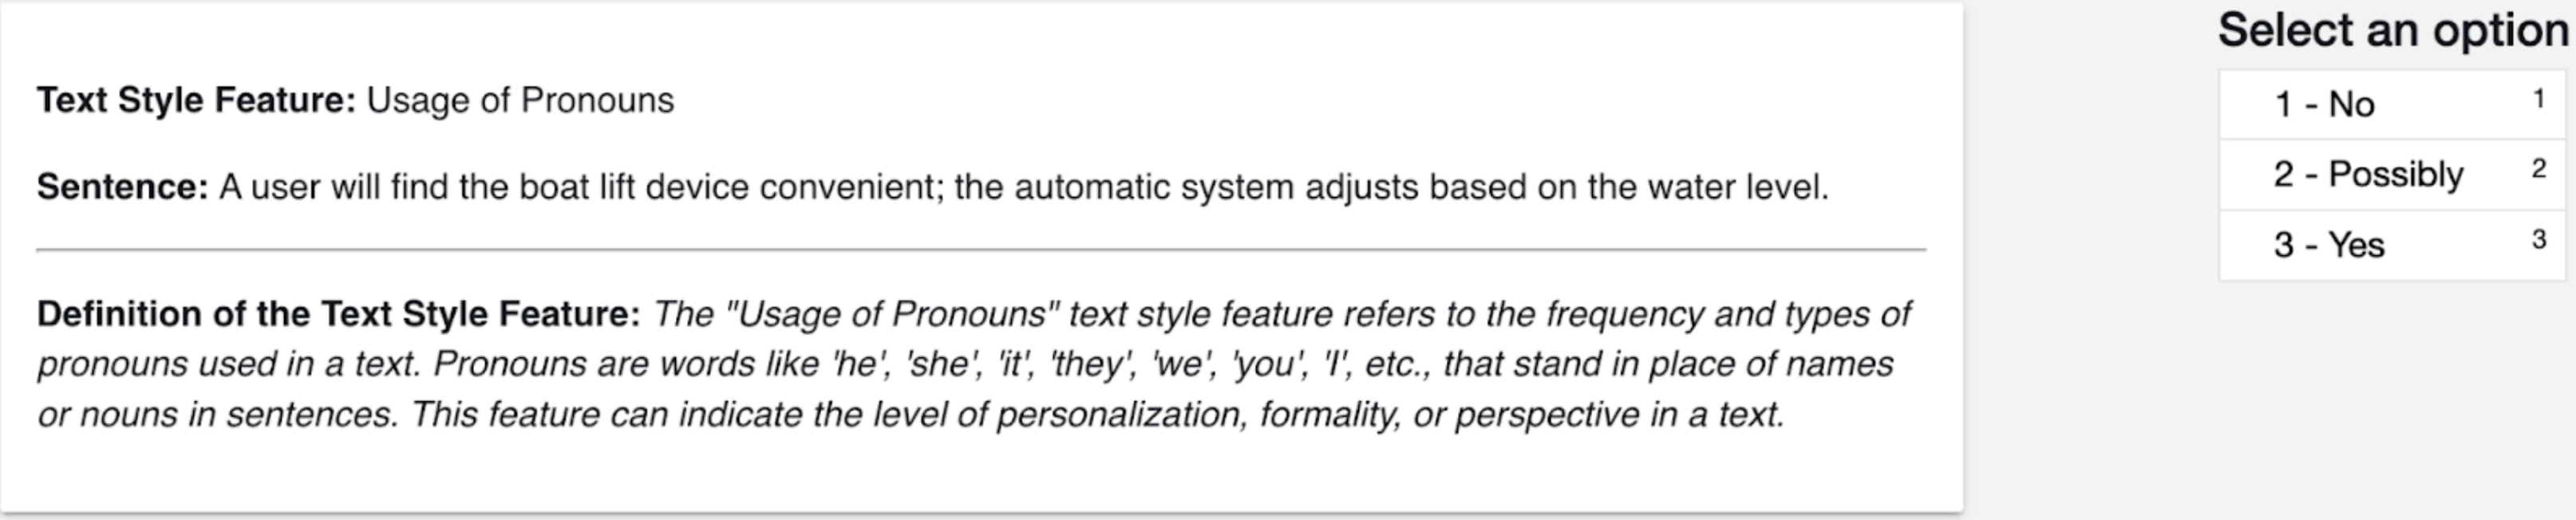
\includegraphics[width=.9\linewidth]{resources/figures/mturkinterface.png}
        \caption{The annotation interface used for human annotation.}
        \label{fig:mturkinterface}
    \end{figure}
}

\input{resources/figures/stylefeaturecategories}

\newcommand{\umapfig}{
    \begin{figure}[H]
        \centering
        \begin{minipage}[b]{0.30\linewidth}
            \centering
            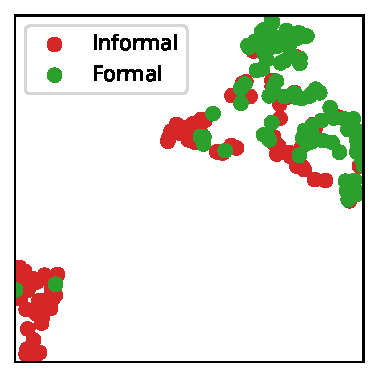
\includegraphics[width=\linewidth]{resources/figures/wegmann_umap.pdf}
            \caption*{\citet{styleemb}}
        \end{minipage}
        \hspace{.1\linewidth}
        \begin{minipage}[b]{0.30\linewidth}
            \centering
            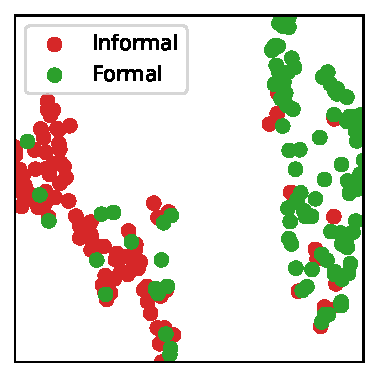
\includegraphics[width=\linewidth]{resources/figures/styledistance_umap.pdf}
            \caption*{\textsc{StyleDistance}}
        \end{minipage}
        \caption{UMAP visualizations of style embeddings from \citet{styleemb} and \textsc{StyleDistance} on $n=100$ random parallel formal/informal examples. \citet{styleemb} forms two distinct clusters of informal texts, making many informal examples distant in the embedding space despite sharing the same style.}
        \label{fig:umapcomparison}
    \end{figure}
}


\newcommand{\stelfig}{
    \begin{figure}[!h]
        \centering
        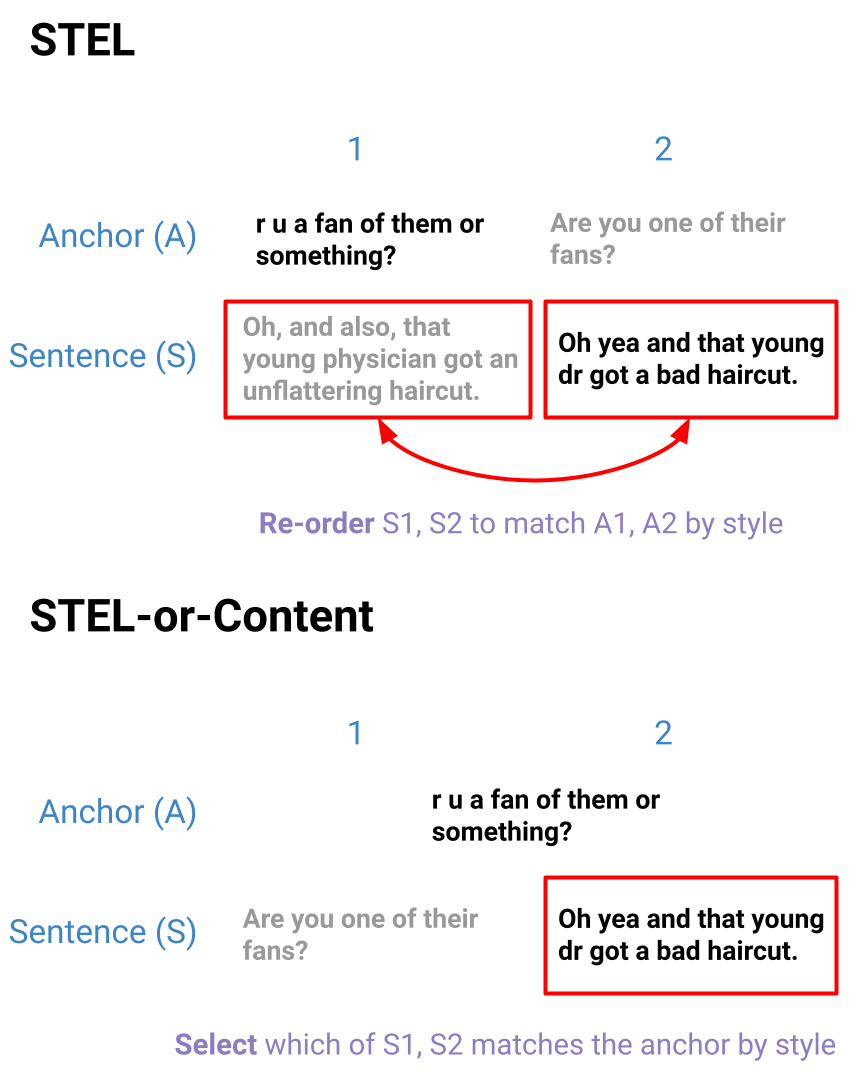
\includegraphics[width=215px]{resources/figures/STELFigure.png}
        % \begin{tikzpicture}
        %     \node[rectangle,
        %         draw = lightgray,
        %         text = black,
        %         fill = lightgray,
        %         minimum width = 215px, 
        %         minimum height = 270px] (r) at (0,0) {Main Figure};
        % \end{tikzpicture}
        \caption{A visualization of the STEL and STEL-or-Content task evaluation we describe in Section \ref{sec:steleval}.}
        \label{fig:stel}
    \end{figure}
}